\documentclass[11pt,a4paper]{article}
\usepackage[T1]{fontenc}
\usepackage[utf8]{inputenc}
\usepackage{lmodern}
\usepackage[margin=2.5cm]{geometry}
\usepackage{amsmath}
\usepackage{graphicx}
\usepackage{booktabs}
\usepackage{array}
\usepackage[section]{placeins}
\usepackage{caption}
\usepackage{enumitem}
\usepackage[hidelinks]{hyperref}
\usepackage{xurl}
\captionsetup{font=small,labelfont=bf}
\setlist{itemsep=2pt,topsep=4pt}
\expandafter\def\csname res@Tc\endcsname{3272}
\expandafter\def\csname res@altApForty\endcsname{227}
\expandafter\def\csname res@altApTwenty\endcsname{190}
\expandafter\def\csname res@altGainHigh\endcsname{1.3}
\expandafter\def\csname res@altGainLow\endcsname{2.4}
\expandafter\def\csname res@altVForty\endcsname{240\,000}
\expandafter\def\csname res@altVTwenty\endcsname{4\,500}
\expandafter\def\csname res@altVolRatioHigh\endcsname{8.9}
\expandafter\def\csname res@altVolRatioLow\endcsname{6.0}
\expandafter\def\csname res@atmP\endcsname{1197}
\expandafter\def\csname res@atmRho\endcsname{0.0184}
\expandafter\def\csname res@atmT\endcsname{226.5}
\expandafter\def\csname res@audDiv\endcsname{60.45}
\expandafter\def\csname res@audDvBack\endcsname{2173}
\expandafter\def\csname res@audDvPct\endcsname{24}
\expandafter\def\csname res@audEratio\endcsname{34}
\expandafter\def\csname res@audGasRatio\endcsname{11.5}
\expandafter\def\csname res@audH2ratio\endcsname{70}
\expandafter\def\csname res@audLnA\endcsname{0.916}
\expandafter\def\csname res@audLnB\endcsname{1.253}
\expandafter\def\csname res@audMolar\endcsname{947}
\expandafter\def\csname res@audPratio\endcsname{9.8}
\expandafter\def\csname res@audRhoLow\endcsname{1.8}
\expandafter\def\csname res@audRhoRatio\endcsname{10.4}
\expandafter\def\csname res@audRhoTot\endcsname{56}
\expandafter\def\csname res@audVolRatio\endcsname{6.1}
\expandafter\def\csname res@balAp\endcsname{214}
\expandafter\def\csname res@balArea\endcsname{4347}
\expandafter\def\csname res@balBareH2\endcsname{22.5}
\expandafter\def\csname res@balBareV\endcsname{17\,600}
\expandafter\def\csname res@balDv\endcsname{2091}
\expandafter\def\csname res@balEnv\endcsname{130}
\expandafter\def\csname res@balEps\endcsname{36.4}
\expandafter\def\csname res@balF\endcsname{11.8}
\expandafter\def\csname res@balH2\endcsname{34.5}
\expandafter\def\csname res@balHb\endcsname{58.0}
\expandafter\def\csname res@balHe\endcsname{75.4}
\expandafter\def\csname res@balHeMassRatio\endcsname{2.18}
\expandafter\def\csname res@balHeVolPct\endcsname{10}
\expandafter\def\csname res@balIsp\endcsname{303.4}
\expandafter\def\csname res@balIspVac\endcsname{307.3}
\expandafter\def\csname res@balLaunchH2\endcsname{38}
\expandafter\def\csname res@balLd\endcsname{8}
\expandafter\def\csname res@balLg\endcsname{369}
\expandafter\def\csname res@balMdot\endcsname{3.97}
\expandafter\def\csname res@balPe\endcsname{4.7}
\expandafter\def\csname res@balQ\endcsname{1.7}
\expandafter\def\csname res@balTap\endcsname{222}
\expandafter\def\csname res@balTb\endcsname{38.1}
\expandafter\def\csname res@balV\endcsname{27\,000}
\expandafter\def\csname res@balVHe\endcsname{29\,600}
\expandafter\def\csname res@balVHi\endcsname{30\,300}
\expandafter\def\csname res@balVLo\endcsname{24\,000}
\expandafter\def\csname res@balVb\endcsname{1714}
\expandafter\def\csname res@betaBase\endcsname{2397}
\expandafter\def\csname res@betaHi\endcsname{4506}
\expandafter\def\csname res@betaLo\endcsname{1046}
\expandafter\def\csname res@bmCstar\endcsname{1726}
\expandafter\def\csname res@bmFrozen\endcsname{274.9}
\expandafter\def\csname res@bmShift\endcsname{285.9}
\expandafter\def\csname res@bmTc\endcsname{3426}
\expandafter\def\csname res@cBalD\endcsname{0.31}
\expandafter\def\csname res@cBalDry\endcsname{90.4}
\expandafter\def\csname res@cBalEnv\endcsname{89}
\expandafter\def\csname res@cBalF\endcsname{5.5}
\expandafter\def\csname res@cBalGas\endcsname{19.3}
\expandafter\def\csname res@cBalM\endcsname{140}
\expandafter\def\csname res@cBalMSS\endcsname{168}
\expandafter\def\csname res@cBalMp\endcsname{49.6}
\expandafter\def\csname res@cBalTb\endcsname{27.1}
\expandafter\def\csname res@cBalV\endcsname{15\,100}
\expandafter\def\csname res@cGndM\endcsname{348}
\expandafter\def\csname res@cGndMSS\endcsname{755}
\expandafter\def\csname res@cGndMp\endcsname{222}
\expandafter\def\csname res@cMassRatio\endcsname{2.5}
\expandafter\def\csname res@cPropRatio\endcsname{4.5}
\expandafter\def\csname res@cSysBal\endcsname{280}
\expandafter\def\csname res@cTwentyM\endcsname{152}
\expandafter\def\csname res@cTwentyV\endcsname{2\,500}
\expandafter\def\csname res@cstar\endcsname{1720}
\expandafter\def\csname res@deaCdFit\endcsname{1.16}
\expandafter\def\csname res@deaD\endcsname{0.171}
\expandafter\def\csname res@deaDragShare\endcsname{8}
\expandafter\def\csname res@deaErrCold\endcsname{+6.2}
\expandafter\def\csname res@deaErrMaxAbs\endcsname{2.6}
\expandafter\def\csname res@deaErrMean\endcsname{+1.3}
\expandafter\def\csname res@deaGroundHeavy\endcsname{22}
\expandafter\def\csname res@deaGroundLight\endcsname{25}
\expandafter\def\csname res@deaImp\endcsname{87.5}
\expandafter\def\csname res@deaIsp\endcsname{191}
\expandafter\def\csname res@deaMp\endcsname{46.7}
\expandafter\def\csname res@deaRmsFit\endcsname{0.8}
\expandafter\def\csname res@deaRmsUnit\endcsname{1.4}
\expandafter\def\csname res@decAltTenBal\endcsname{127}
\expandafter\def\csname res@decAltTenDrag\endcsname{63}
\expandafter\def\csname res@decAltTenGnd\endcsname{35}
\expandafter\def\csname res@decAltTenHead\endcsname{11}
\expandafter\def\csname res@decAltTenNozzle\endcsname{26}
\expandafter\def\csname res@decAltTenRatio\endcsname{3.7}
\expandafter\def\csname res@decAltTwentyBal\endcsname{190}
\expandafter\def\csname res@decAltTwentyDrag\endcsname{56}
\expandafter\def\csname res@decAltTwentyGnd\endcsname{35}
\expandafter\def\csname res@decAltTwentyHead\endcsname{13}
\expandafter\def\csname res@decAltTwentyNozzle\endcsname{31}
\expandafter\def\csname res@decAltTwentyRatio\endcsname{5.5}
\expandafter\def\csname res@decDrag\endcsname{93}
\expandafter\def\csname res@decFDrag\endcsname{52}
\expandafter\def\csname res@decFHead\endcsname{17}
\expandafter\def\csname res@decFNozzle\endcsname{31}
\expandafter\def\csname res@decHead\endcsname{31}
\expandafter\def\csname res@decMassBigBal\endcsname{203}
\expandafter\def\csname res@decMassBigDrag\endcsname{41}
\expandafter\def\csname res@decMassBigGnd\endcsname{60}
\expandafter\def\csname res@decMassBigHead\endcsname{22}
\expandafter\def\csname res@decMassBigNozzle\endcsname{37}
\expandafter\def\csname res@decMassBigRatio\endcsname{3.4}
\expandafter\def\csname res@decMassFiftyBal\endcsname{221}
\expandafter\def\csname res@decMassFiftyDrag\endcsname{60}
\expandafter\def\csname res@decMassFiftyGnd\endcsname{18}
\expandafter\def\csname res@decMassFiftyHead\endcsname{15}
\expandafter\def\csname res@decMassFiftyNozzle\endcsname{24}
\expandafter\def\csname res@decMassFiftyRatio\endcsname{12.4}
\expandafter\def\csname res@decNozzle\endcsname{56}
\expandafter\def\csname res@dryFor100\endcsname{269}
\expandafter\def\csname res@dvCap\endcsname{991}
\expandafter\def\csname res@dvCapOpt\endcsname{1235}
\expandafter\def\csname res@fallAp\endcsname{181}
\expandafter\def\csname res@fallCost\endcsname{33}
\expandafter\def\csname res@fallDv\endcsname{2086}
\expandafter\def\csname res@fallEps\endcsname{36.4}
\expandafter\def\csname res@fallF\endcsname{11.8}
\expandafter\def\csname res@fallHb\endcsname{51.5}
\expandafter\def\csname res@fallIsp\endcsname{302.8}
\expandafter\def\csname res@fallIspVac\endcsname{307.3}
\expandafter\def\csname res@fallLd\endcsname{10}
\expandafter\def\csname res@fallLg\endcsname{369}
\expandafter\def\csname res@fallMdot\endcsname{3.98}
\expandafter\def\csname res@fallPe\endcsname{4.7}
\expandafter\def\csname res@fallQ\endcsname{2.2}
\expandafter\def\csname res@fallSpeed\endcsname{139}
\expandafter\def\csname res@fallTap\endcsname{205}
\expandafter\def\csname res@fallTb\endcsname{38.0}
\expandafter\def\csname res@fallVb\endcsname{1567}
\expandafter\def\csname res@feedAl\endcsname{0.211}
\expandafter\def\csname res@feedSS\endcsname{0.477}
\expandafter\def\csname res@filmAreal\endcsname{18.4}
\expandafter\def\csname res@frDeficitPct\endcsname{15}
\expandafter\def\csname res@frDel\endcsname{246}
\expandafter\def\csname res@frFrozen\endcsname{241.4}
\expandafter\def\csname res@frShift\endcsname{267.9}
\expandafter\def\csname res@frTc\endcsname{1443}
\expandafter\def\csname res@ftAl\endcsname{0.060}
\expandafter\def\csname res@ftHP\endcsname{1.97}
\expandafter\def\csname res@ftSS\endcsname{0.237}
\expandafter\def\csname res@gainKm\endcsname{179}
\expandafter\def\csname res@gainRatio\endcsname{6.2}
\expandafter\def\csname res@gasH2\endcsname{0.0748}
\expandafter\def\csname res@gasHe\endcsname{0.160}
\expandafter\def\csname res@gndAp\endcsname{35}
\expandafter\def\csname res@gndDv\endcsname{1636}
\expandafter\def\csname res@gndEps\endcsname{3.68}
\expandafter\def\csname res@gndF\endcsname{11.8}
\expandafter\def\csname res@gndFirstTen\endcsname{9.2}
\expandafter\def\csname res@gndHb\endcsname{11.7}
\expandafter\def\csname res@gndIsp\endcsname{226.4}
\expandafter\def\csname res@gndIspVac\endcsname{259.0}
\expandafter\def\csname res@gndLd\endcsname{508}
\expandafter\def\csname res@gndLg\endcsname{278}
\expandafter\def\csname res@gndMdot\endcsname{5.32}
\expandafter\def\csname res@gndPe\endcsname{106.0}
\expandafter\def\csname res@gndQ\endcsname{121}
\expandafter\def\csname res@gndTap\endcsname{95}
\expandafter\def\csname res@gndTb\endcsname{28.4}
\expandafter\def\csname res@gndVb\endcsname{850}
\expandafter\def\csname res@h2oRatio\endcsname{6}
\expandafter\def\csname res@heBottleHi\endcsname{2.6}
\expandafter\def\csname res@heBottleKg\endcsname{0.113}
\expandafter\def\csname res@heBottleLo\endcsname{1.4}
\expandafter\def\csname res@heBottleMid\endcsname{1.8}
\expandafter\def\csname res@heKg\endcsname{0.0085}
\expandafter\def\csname res@heMassHi\endcsname{50}
\expandafter\def\csname res@heMassLo\endcsname{26}
\expandafter\def\csname res@heMassMid\endcsname{34}
\expandafter\def\csname res@heVolHi\endcsname{872}
\expandafter\def\csname res@heVolLo\endcsname{453}
\expandafter\def\csname res@heVolMid\endcsname{597}
\expandafter\def\csname res@ispDel\endcsname{307.3}
\expandafter\def\csname res@ispDelHi\endcsname{317}
\expandafter\def\csname res@ispDelLo\endcsname{284}
\expandafter\def\csname res@ispFrozen\endcsname{312.9}
\expandafter\def\csname res@ispFrozenPeak\endcsname{315.0}
\expandafter\def\csname res@ispShift\endcsname{334.0}
\expandafter\def\csname res@ispShiftPeak\endcsname{335.8}
\expandafter\def\csname res@lapP\endcsname{270}
\expandafter\def\csname res@lapRho\endcsname{0.0101}
\expandafter\def\csname res@lapT\endcsname{93.45}
\expandafter\def\csname res@lapZero\endcsname{44}
\expandafter\def\csname res@mapApTen\endcsname{127}
\expandafter\def\csname res@mcBalCv\endcsname{9}
\expandafter\def\csname res@mcBalHi\endcsname{238}
\expandafter\def\csname res@mcBalLo\endcsname{176}
\expandafter\def\csname res@mcBalMed\endcsname{204}
\expandafter\def\csname res@mcDragLargest\endcsname{100}
\expandafter\def\csname res@mcFDragHi\endcsname{56}
\expandafter\def\csname res@mcFDragLo\endcsname{46}
\expandafter\def\csname res@mcFDragMed\endcsname{51}
\expandafter\def\csname res@mcFHeadHi\endcsname{21}
\expandafter\def\csname res@mcFHeadLo\endcsname{16}
\expandafter\def\csname res@mcFHeadMed\endcsname{18}
\expandafter\def\csname res@mcFNozzleHi\endcsname{34}
\expandafter\def\csname res@mcFNozzleLo\endcsname{27}
\expandafter\def\csname res@mcFNozzleMed\endcsname{30}
\expandafter\def\csname res@mcGndCv\endcsname{18}
\expandafter\def\csname res@mcGndHi\endcsname{43}
\expandafter\def\csname res@mcGndLo\endcsname{24}
\expandafter\def\csname res@mcGndMed\endcsname{32}
\expandafter\def\csname res@mcN\endcsname{10\,000}
\expandafter\def\csname res@mcNshap\endcsname{1\,000}
\expandafter\def\csname res@mcPbelow\endcsname{0.0}
\expandafter\def\csname res@mcRatioHi\endcsname{8.0}
\expandafter\def\csname res@mcRatioLo\endcsname{5.0}
\expandafter\def\csname res@mcRatioMed\endcsname{6.3}
\expandafter\def\csname res@mpFor100\endcsname{82}
\expandafter\def\csname res@mrCap\endcsname{1.51}
\expandafter\def\csname res@nacaMassHi\endcsname{106}
\expandafter\def\csname res@nacaMassLo\endcsname{86}
\expandafter\def\csname res@ofFrozenPeak\endcsname{2.05}
\expandafter\def\csname res@ofShiftPeak\endcsname{2.75}
\expandafter\def\csname res@peakAccel\endcsname{8.1}
\expandafter\def\csname res@propFrac\endcsname{0.502}
\expandafter\def\csname res@propH2Ratio\endcsname{7.5}
\expandafter\def\csname res@propRhoOwn\endcsname{0.099}
\expandafter\def\csname res@propVolL\endcsname{156}
\expandafter\def\csname res@propVolRatio\endcsname{9.4}
\expandafter\def\csname res@rhoBalCd\endcsname{-0.02}
\expandafter\def\csname res@rhoBalDry\endcsname{-0.70}
\expandafter\def\csname res@rhoBalEta\endcsname{+0.66}
\expandafter\def\csname res@rhoBalTw\endcsname{+0.20}
\expandafter\def\csname res@rhoBalZf\endcsname{+0.10}
\expandafter\def\csname res@rhoGndCd\endcsname{-0.70}
\expandafter\def\csname res@rhoGndDry\endcsname{-0.31}
\expandafter\def\csname res@rhoGndEta\endcsname{+0.58}
\expandafter\def\csname res@rhoGndTw\endcsname{-0.23}
\expandafter\def\csname res@rhoGndZf\endcsname{-0.01}
\expandafter\def\csname res@rhoH2float\endcsname{0.00128}
\expandafter\def\csname res@runBBB\endcsname{214}
\expandafter\def\csname res@runBBG\endcsname{144}
\expandafter\def\csname res@runBGB\endcsname{106}
\expandafter\def\csname res@runBGG\endcsname{65}
\expandafter\def\csname res@runGBB\endcsname{182}
\expandafter\def\csname res@runGBG\endcsname{112}
\expandafter\def\csname res@runGGB\endcsname{75}
\expandafter\def\csname res@runGGG\endcsname{35}
\expandafter\def\csname res@sCdHi\endcsname{212}
\expandafter\def\csname res@sCdLo\endcsname{215}
\expandafter\def\csname res@sEtaHi\endcsname{227}
\expandafter\def\csname res@sEtaLo\endcsname{185}
\expandafter\def\csname res@sGndCdHi\endcsname{28}
\expandafter\def\csname res@sGndCdLo\endcsname{43}
\expandafter\def\csname res@sGndD30\endcsname{58}
\expandafter\def\csname res@sGndD35\endcsname{45}
\expandafter\def\csname res@sTwHi\endcsname{221}
\expandafter\def\csname res@sTwLo\endcsname{176}
\expandafter\def\csname res@suiApHeavy\endcsname{60}
\expandafter\def\csname res@suiApLight\endcsname{91}
\expandafter\def\csname res@suiFire\endcsname{11.6}
\expandafter\def\csname res@suiMassFit\endcsname{103}
\expandafter\def\csname res@suiMassHi\endcsname{103}
\expandafter\def\csname res@suiMassLo\endcsname{107}
\expandafter\def\csname res@suiMassMid\endcsname{105}
\expandafter\def\csname res@suiTop\endcsname{61}
\expandafter\def\csname res@tankHP\endcsname{299}
\expandafter\def\csname res@tankHPsf\endcsname{219}
\expandafter\def\csname res@vmin\endcsname{1161}

\makeatletter\newcommand{\tabin}[1]{\@@input #1 }\makeatother
\newcommand{\R}[1]{\csname res@#1\endcsname}
\newcommand{\Isp}{I_{\mathrm{sp}}}
\newcommand{\ms}{\,\mathrm{m\,s^{-1}}}
\newcommand{\kgm}{\,\mathrm{kg\,m^{-3}}}

\title{\textbf{Supplementary material: audit of the 2022 Project AKS proposal, and hazards and regulation}}
\author{Aadi Ramnani \and Karthikeya Aduru \and Bala Mysura Sreethan Reddy}
\date{Supplement to ``The mass-optimal float altitude for balloon-launched sounding rockets is robust; the mass saving is not''}
\begin{document}
\maketitle
\noindent Numbers in this supplement are generated by the same scripts as the paper and read from the same \texttt{results.tex}. Section numbers refer to the paper.

\begin{figure}[!htb]
\centering
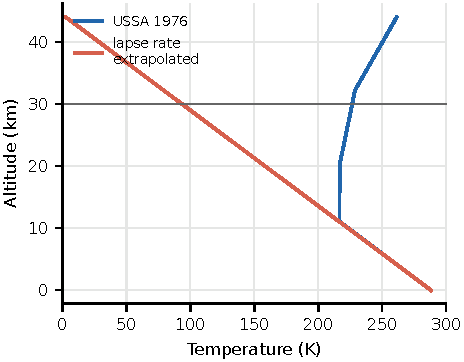
\includegraphics[width=0.48\textwidth]{../paper/figures/fig_lapse.pdf}
\caption{Temperature of the U.S. Standard Atmosphere 1976 and of the tropospheric lapse rate extrapolated above 11\,km, as used in the 2022 proposal.}
\label{fig:lapse}
\end{figure}

\section*{Audit of the 2022 proposal}


Project AKS was a proposal that we wrote in 2022--23. It described a 301.27\,kg rocket (150\,kg dry, 151.27\,kg of propellant) burning UDMH and N$_2$O$_4$, carried by a hydrogen balloon to about 30\,km and ignited at about 29\,km after the balloon burst, with a target apogee of 100\,km. It was presented to our school principal and went no further; no hardware was built and no tests were made. The original document is available from the authors. We recomputed every step of it. Table~\ref{tab:audit} lists the errors and the check that would have caught each one. The main points are these.

\emph{Rocket equation.} With a final mass of 150\,kg and an initial mass of $150+\tfrac52 m_{\mathrm{ox}}$, the mass ratio still contains the unknown oxidizer mass. The proposal replaced it by the constant $1+\tfrac52$, evaluated $\ln(1+\tfrac52)$ as $\ln 2.5=\R{audLnA}$ instead of $\ln 3.5=\R{audLnB}$, and obtained $\Delta v=2854.7\ms$. With the proposal's own final masses and specific impulse the rocket equation gives \R{audDvBack}$\ms$, \R{audDvPct}\% less. Nothing connected $\Delta v$ to the target altitude; the minimum drag-free burnout speed for a coast from 30 to 100\,km is \R{vmin}$\ms$.

\emph{Atmosphere and balloon.} The proposal extrapolated the tropospheric lapse rate of $6.49\,\mathrm{K\,km^{-1}}$ to 30\,km and obtained \R{lapT}\,K; the standard value is \R{atmT}\,K, and the linear model reaches absolute zero at \R{lapZero}\,km (Fig.~\ref{fig:lapse}). With that temperature the barometric formula gives \R{lapP}\,Pa, but 2654.98\,Pa was reported. The density was reported as 1.03$\kgm$, whereas the proposal's own pressure and temperature give \R{propRhoOwn}$\kgm$; the standard value is \R{atmRho}$\kgm$, \R{audRhoTot} times smaller than the figure used. The volume was then computed as a weight in newtons divided by a density, and the hydrogen mass from the density of hydrogen at 0\,$^\circ$C and 1\,atm, which is \R{audH2ratio} times its density at float. These errors partly cancel. The reported volume (2870\,m$^3$) is \R{audVolRatio} times too small for the bare rocket and the reported hydrogen mass (258\,kg) \R{audGasRatio} times too large. Against the complete balloon of the baseline vehicle (Sec.~S2.4 of the supplement on the apogee gain) the volume is \R{propVolRatio} times too small and the hydrogen mass \R{propH2Ratio} times too large. Because the final answer looked plausible, nothing prompted a second look.

\emph{Propellant.} The proposal applied the propellants at $\mathrm{O/F}=0.67$ and took its specific impulse, 316.7\,s, from a study of aluminium-loaded UDMH gels at other mixture ratios \cite{varghese1999}. For neat propellants at $\mathrm{O/F}=0.67$ our gas-phase equilibrium calculation gives a chamber temperature of \R{frTc}\,K and an ideal vacuum specific impulse of \R{frShift}\,s, \R{frDeficitPct}\% below the value assumed. That calculation neglects condensed carbon and assumes equilibrium at a temperature where the chemistry is slow, so it is an upper estimate.

\emph{Tanks.} The proposal specified stainless-steel tanks at 3000\,psi (20.7\,MPa) inside a 150\,kg dry mass. By the relation of Sec.~2.7 of the paper, ideal spheres for the \R{propVolL}\,L of propellant weigh \R{tankHP}\,kg (\R{tankHPsf}\,kg with a safety factor of only 1.1), which is \R{ftHP}\,kg per kilogram of propellant. Tanks of this kind limit the mass ratio to \R{mrCap} however much propellant is carried. With a delivered specific impulse of \R{frDel}\,s at $\mathrm{O/F}=0.67$ the ideal $\Delta v$ is then at most \R{dvCap}$\ms$, below the \R{vmin}$\ms$ needed, so the design could not reach 100\,km even with an instantaneous burn and no other dry mass. The specified 5000\,psi (34.5\,MPa) helium bottle would weigh \R{heBottleLo}--\R{heBottleHi}\,t in the same steel, for end pressures of 22--28\,MPa.

\emph{What survives.} With the proposed 150\,kg dry mass and the propulsion of Sec.~2.3 of the paper, \R{mpFor100}\,kg of propellant would reach 100\,km from 30\,km, and with the proposed 151\,kg of propellant the dry mass could grow to \R{dryFor100}\,kg. The idea of igniting above most of the atmosphere was sound. What failed was the tank and pressurant specification and the choice of propellants.

\begin{table}[p]
\centering
\caption{Errors in the 2022 proposal and the check that would have caught each one.}
\label{tab:audit}
\footnotesize
\begin{tabular}{@{}l>{\raggedright\arraybackslash}p{5.0cm}>{\raggedright\arraybackslash}p{2.0cm}>{\raggedright\arraybackslash}p{3.6cm}>{\raggedright\arraybackslash}p{3.2cm}@{}}
\toprule
\# & Error & Class & Effect & Check \\
\midrule
E1 & Mass ratio $(150+\tfrac52 m_{\mathrm{ox}})/150$ replaced by the constant $1+\tfrac52$ & Algebra & $\Delta v$ made independent of the propellant load & Keep the unknown symbolic to the end \\
E2 & $\ln(1+\tfrac52)$ evaluated as $\ln 2.5$ & Arithmetic & $\Delta v$ too low by a factor 0.73 & Recompute \\
E3 & Quoted $\Delta v$ (2855$\ms$) inconsistent with final masses (\R{audDvBack}$\ms$) & Consistency & Propellant and $\Delta v$ do not match & Back-substitute the final answer \\
E4 & No $\Delta v$ requirement derived from the 100\,km target & Missing model & Propellant load not tied to the mission & Energy bound plus gravity loss \\
E5 & Invalid rearrangement; $226.215/3.7419=\R{audDiv}\neq 60.51$ & Algebra, arithmetic & Oxidizer mass unsupported & Back-substitute \\
E6 & Tropospheric lapse rate used up to 30\,km & Model outside its range & \R{lapT}\,K instead of \R{atmT}\,K; density \R{audRhoLow} times too low & Check the validity range \\
E7 & Barometric formula gives \R{lapP}\,Pa; 2655\,Pa reported & Arithmetic & \R{audPratio} times the formula's own value & Recompute \\
E8 & Density \R{propRhoOwn}$\kgm$ reported as 1.03$\kgm$ & Arithmetic & \R{audRhoRatio} times the value from its own inputs & Compare with sea level (1.225$\kgm$) \\
E9 & Volume computed as weight / density & Dimensional & Factor 9.81; units m$^4$\,s$^{-2}$ & Carry units through every line \\
E10 & Hydrogen density at 0\,$^\circ$C and 1\,atm applied at 30\,km & Reference state & Gas mass \R{audH2ratio} times too high & Evaluate all densities at one state \\
E11 & Molar volume written as 22.414\,m$^3$\,mol$^{-1}$ & Units & Intermediate result does not follow & Carry units \\
E12 & $\Isp$ of aluminised gels applied to neat propellants at $\mathrm{O/F}=0.67$ & Data provenance & $\Isp$ overstated by about \R{frDeficitPct}\% & Check the conditions behind every datum \\
E13 & 20.7\,MPa steel tanks inside a 150\,kg dry mass & Mass closure & Tanks about \R{tankHP}\,kg & Pressure-vessel scaling \\
E14 & Suborbital cost per kg compared with orbital prices \cite{jones2018}; currency conversion off by ten & Category, arithmetic & Cost claim unsupported & Compare like with like \\
E15 & Pressure-fed text, pump-fed diagrams; bell and aerospike nozzles & Internal consistency & No single design to analyse & One design, one parts list \\
E16 & Hazards understated (``only one hazard'', ``foolproof'') & Safety data & Unsafe framing & Consult exposure limits (see the hazards section below) \\
\bottomrule
\end{tabular}
\end{table}

On E14: lifting 1\,kg to 100\,km from rest takes about $1/\R{audEratio}$ of the specific energy of a 400\,km circular orbit, so the two prices are not comparable. The proposal also stated that the vehicle would be the highest-flying student-led rocket. That was already untrue when it was written: the University of Southern California's Traveler~IV reached 339\,800\,ft in April 2019 \cite{traveler}.

\section*{Hazards and regulation}


The hazards that led us to close the project are more serious than the proposal acknowledged. UDMH is classified by IARC in Group 2B, possibly carcinogenic to humans \cite{iarc}. NIOSH lists it as a potential occupational carcinogen with a recommended exposure limit of 0.06\,ppm (2-hour ceiling) and an immediately-dangerous concentration of 15\,ppm; its vapour pressure is 103\,mmHg, about \R{h2oRatio} times that of water at 20\,$^\circ$C, its flash point is 5\,$^\circ$F, and its flammable range is 2--95\% by volume \cite{nioshudmh}. Nitrogen tetroxide is in equilibrium with nitrogen dioxide, for which NIOSH gives a short-term limit of 1\,ppm and an immediately-dangerous concentration of 13\,ppm \cite{nioshno2}. Hydrogen is flammable over a wide range of concentrations in air, and the balloon of the baseline vehicle (Sec.~S2.4 of the supplement on the apogee gain) would hold about \R{balLaunchH2}\,kg of it. Professional programmes handle these materials with protective equipment, trained staff and dedicated facilities, none of which a school can provide. Closing the project was the right decision.

A flight in India would also have needed, at a minimum, authorisation from the Indian National Space Promotion and Authorisation Centre \cite{inspace}, airspace clearance under the Bharatiya Vayuyan Adhiniyam, 2024 \cite{bva}, approvals for pressure vessels and gas cylinders \cite{peso}, and compliance with the rules on hazardous chemicals \cite{msihc}. We have not assessed which provisions would apply.

\begin{thebibliography}{99}

\bibitem{varghese1999} T.\,L. Varghese, N. Prabhakaran, K.\,P. Thanki, S. Subramanian, S.\,S. Rao, K.\,N. Ninan, and V.\,N. Krishnamurthy, ``Performance evaluation and experimental studies on metallised gel propellants,'' Def. Sci. J. \textbf{49}, 71--78 (1999).

\bibitem{jones2018} H.\,W. Jones, ``The recent large reduction in space launch cost,'' in \emph{48th International Conference on Environmental Systems}, ICES-2018-81 (Albuquerque, NM, 2018).

\bibitem{traveler} A. Aitoumeziane, P. Eusebio, C. Hayes, V. Ramachandran, J. Smith, J. Sridharan, L. St.~Regis, M. Stephenson, N. Tewksbury, M. Tran, and H. Yang, ``Traveler IV apogee analysis,'' white paper (USC Rocket Propulsion Laboratory, Los Angeles, May 2019), \url{http://www.uscrpl.com/s/Traveler-IV-Whitepaper}.

\bibitem{iarc} International Agency for Research on Cancer, \emph{IARC Monographs on the Evaluation of Carcinogenic Risks to Humans, Vol.~71: Re-evaluation of Some Organic Chemicals, Hydrazine and Hydrogen Peroxide} (IARC, Lyon, 1999).

\bibitem{nioshudmh} National Institute for Occupational Safety and Health, ``NIOSH Pocket Guide to Chemical Hazards: 1,1-Dimethylhydrazine,'' \url{https://www.cdc.gov/niosh/npg/npgd0227.html} (accessed 18 November 2026).

\bibitem{nioshno2} National Institute for Occupational Safety and Health, ``NIOSH Pocket Guide to Chemical Hazards: Nitrogen dioxide,'' \url{https://www.cdc.gov/niosh/npg/npgd0454.html} (accessed 18 November 2026).

\bibitem{inspace} Indian National Space Promotion and Authorisation Centre, \emph{Norms, Guidelines and Procedures for Implementation of Indian Space Policy-2023 in respect of Authorization of Space Activities}, IN:ISP2023:NGP2024/V1.0 (IN-SPACe, Ahmedabad, 2024).

\bibitem{bva} Government of India, \emph{The Bharatiya Vayuyan Adhiniyam, 2024}, Act No.~16 of 2024.

\bibitem{peso} Government of India, \emph{The Static and Mobile Pressure Vessels (Unfired) Rules, 2016}, G.S.R. 1109(E), and \emph{The Gas Cylinders Rules, 2016}, G.S.R. 1081(E).

\bibitem{msihc} Government of India, \emph{The Manufacture, Storage and Import of Hazardous Chemical Rules, 1989}, S.O. 966(E), under the Environment (Protection) Act, 1986.

\end{thebibliography}
\end{document}
